\section{Grundlagen zur Bearbeitung}
Für das Projektverständnis sind Grundlagen zu schaffen. Sowohl die Einordnung des Projektthemas
als auch die unterschiedlichen Tools, Informationssysteme und genutzten Methoden müssen verständlich erläutert sein, um den Gesamtkontext der Arbeit einordnen zu können.

\subsection{Inbound Marketing}
Inbound Marketing ist eine Art des Marketings, die auf personalisierter Werbung besteht und den Kunden zum Unternehmen bringen soll. Der Kunde soll, der Firma gegenüber, loyal und freundlich gesinnt sein. Dies wird durch personalisierte Werbung erreicht, bei welcher der Kunde nicht direkt vom Marketing Team angesprochen wird. Dafür werden Kundendaten benötigt, mit welchen die Firma gezielt Werbung schalten kann. Diese Werbung wird nicht nur auf der eigenen Plattform betrieben, sondern erreicht den Kunden über mehrere Kanäle. Somit bleibt das Unternehmen dem Kunden im Hinterkopf und wenn sich ein Problem entwickelt, bei welchem das Unternehmen eine Lösung anbietet wird sich der Kunde an das  Unternehmen wenden.
\newline 
Allerdings spielt nicht nur Werbung eine große Rolle im Inbound Marketing, da die potenziellen Kunden erst einmal auf das Unternehmen aufmerksam werden müssen. Dies geschieht durch gute Erfahrungen von Bekannten oder Kollegen, genauso wie die Vorstellung der eigenen Leistungen. Dies kann durch die eigene Website sein, Soziale Medien oder Blogs, welche vom Marketing Team gepflegt werden. Wird der potenzielle Kunde durch solche Informationen auf das Unternehmen aufmerksam, kann sich, über Cookies oder ähnliches, das Unternehmen den User merken und ihm gezielt Werbung schalten. Somit bleibt das Unternehmen im Gedächtnis des potenziellen Kunden und sobald dieser eine Leistung benötigt, welche das besagte Unternehmen anbietet, wird er an dieses denken und sich an das Unternehmen wenden. Genauso ist es wichtig bei Suchmaschinen wie 'Google', 'Bing' etc. weit oben zu sein. Dadurch kann der potenzielle Neukunde das Unternehmen schneller entdecken. Des Weiteren besuchen die wenigsten Menschen die zweite oder dritte Seite einer Suchmaschine, weshalb es sehr von Vorteil für ein Unternehmen ist, bei Suchmaschinen weit oben gelistet zu sein.
\newline 
Ein weiterer Teil des Inbound Marketings ist es nicht alle Informationen auf einmal Preis zu geben. Besucht ein potenzieller Kunde eine Website, so kann er meist alle Informationen einsehen. Beim Inbound Marketing wird dem potenziellen Kunden nur ein Bruchteil der möglichen Informationen geliefert. Um an weitere zu kommen ist es notwendig eine Mail Adresse oder andere Daten, welche das Unternehmen weiter für Werbung nutzen kann, zu hinterlegen. Somit kann sich der Kunde weiter informieren und zeigt sein ehrliches Interesse an dem Unternehmen und das Unternehmen erhält nötige Daten, welche für weitere Inbound Marketing Strategien genutzt werden kann. 
\newline 
Damit die Werbung richtig personalisiert werden kann ist es wichtig für das Unternehmen, dass es seine Zielkunden kennt. Hierfür werden 'Buyers Personas' und 'Ideal Customer Profile' angelegt. 
\newline 
Um ein 'Ideal Customer Profil' anzulegen, muss ein Unternehmen wissen, wie die eigenen Kunden ausschauen. Sind es andere Unternehmen, so sollte klar sein, wie viele Angestellte die Kunden im Durchschnitt haben, welches Budget ihnen zur Verfügung steht, wo die Sitze des Unternehmens liegen und wie lange die Projekte oder einzelnen Geschäftsbeziehungen im durchschnitt dauern. Mit Hilfe dieses 'Ideal Customer Profil' können Unternehmen ermitteln, ob ein potenzieller Kunde in das Schema des Unternehmens passt oder ob es die eigene Kapazität übersteigt. Außerdem kann mit dem 'Ideal Customer Profil' ermittelt werden, auf welchen Plattformen die Kunden am besten zu erreichen sind, da große Unternehmen anders operieren, als Mittelständige oder Kleinunternehmen. 
\newline 
Bei den 'Buyers Personas' wird geschaut, wer dafür Zuständig ist die Geschäfte mit der eigenen Firma abzuwickeln. Dabei wird festgestellt, ob es ein Abteilungsleiter oder CEO des Unternehmens ist. Des weiteren wird geschaut, worauf die einzelnen Kunden achten. Dabei werden die bestehenden Kunden analysiert, um festzustellen, wo Gemeinsamkeiten bestehen und inwiefern sich die einzelnen Kunden unterscheiden. Anhand dieser Informationen wird festgestellt, welche Herausforderungen die einzelnen Kunden mit sich bringen und wie diese spezifisch in der Werbung angesprochen werden können, um das eigene Angebot attraktiv zu machen. 
\newline 
Mit Hilfe der Buyers Personas' und 'Ideal Customer Profile', kann das Unternehmen beginnen die eigenen Kunden in Gruppen zu unterteilen. Zu diesen Gruppen werden die potenziellen Neukunden ebenfalls zugewiesen, um die Werbung so individuell und attraktiv wie möglich zu gestalten. Somit kann viel mehr auf die eigenen Interessen der verschiedenen Kunden und Neukunden eingegangen werden. Die bestehenden Kunden haben das Gefühl, dass das Unternehmen genau weiß, was die Kunden brauchen und die möglichen Neukunden zeigen schneller Interesse, da gleich auf die eigenen Probleme und Bedürfnisse eingegangen wird. Sie denken gleich, dass das Unternehmen genau das bieten kann was sie benötigen. 
\newline 
Durch das Inbound Marketing lassen sich gute, lukrative und lange Geschäftsbeziehungen erstellen. Außerdem kann sich das Unternehmen viel besser selbst einschätzen und auch besser auf die Probleme und Herausforderungen der Kunden eingehen. Allerdings kostet Inbound Marketing viel Aufwand als gewöhnliche Marketing Methoden. Es muss spezifisch auf die Kunden eingegangen werden und die Kommunikation zwischen Unternehmen und Kunde steht im Vordergrund, weshalb die Unternehmen um einiges mehr an Arbeit in die Kundenbeziehungen stecken müssen. Seien es die bestehenden Kunden, welche nicht verloren gehen dürfen oder die Neukunden, welche über das Unternehmen selbst informiert werden müssen. Dennoch stechen die positiven Aspekte des Inbound Marketings deutlich heraus und viele Unternehmen, besonders Mittelständige und Start-Up Unternehmen nutzen diese Methode des Marketings um auf sich aufmerksam zu machen.

\subsection{Outbound Marketing}
Unter den Begriff Outbound Marketing fällt fast alles was zu den traditionellen Marketing Methoden zählt. Hier kommt der Kunde nicht zur Firma, sondern die Firma zum Kunden. 
\newline 
Die meisten Methoden des Outbound Marketings sind die bekannten Werbemethoden. Dazu zählen Spam, Kaltakquise, Briefpost, Radiowerbung, TV-Werbung, Flyer oder Vertreter. 
\begin{figure} [H]
	\centering
	\begin{minipage}[b]{.45\linewidth}
		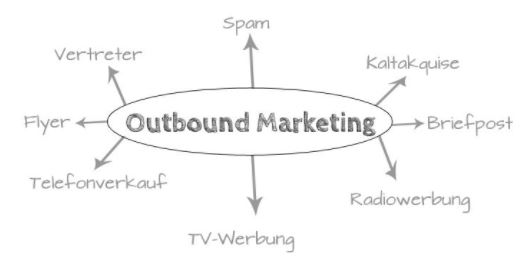
\includegraphics[width=7.5cm]{./Grafiken2/Outbound_Marketing.JPG}
		\caption{Outbound Marketing (/onlinemarketing.de/lexikon/outbound-marketing)}
		\label{Create_Zubereitung}
	\end{minipage}
\end{figure}
Alle diese Methoden haben gemeinsam, dass das Unternehmen sich an den Kunden wendet. Es wird immer eine große Anzahl an Leuten erreicht, jedoch gibt es meist nur wenige die sich überhaupt dafür interessieren, den Beruf ausüben oder Wissen in dem Bereich des Unternehmens haben. Die Strategie hinter diesen Methoden liegt darin, so viele Menschen wie möglich zu erreichen, damit die wenigen welche an dem Produkt interessiert sein könnten ebenfalls die Werbung erhalten. Genauso könnte das Interesse weniger Menschen oder Unternehmen durch diese Methode des Marketings geweckt werden, damit diese das Produkt oder die Dienstleistung des Unternehmens für sich in Anspruch nehmen. 
\newline
Somit gestaltet sich die Neukundenakquise mit Outbound Marketing etwas schwierig, da alle Methoden das Problem haben, zu viele Menschen zu erreichen, die höchstwahrscheinlich nie Kunden werden. Des weiteren kostet es sehr viel Arbeit und Geld, um genug Menschen zu erreichen, damit die richtige Person, die das Produkt oder die Dienstleistung kauft, dabei ist.
\newline 
Eine weitere Methode des Outbound Marketings sind Newsletter oder gezielte Mails an Kunden. Dabei wendet sich das Unternehmen ebenfalls an die Kunden, jedoch in einem viel kleineren Spektrum. Hierbei werden nur Kunden, die auch wirklich an der Dienstleistung oder dem Produkt interessiert sein könnten, diese erhalten. Newsletter müssen abonniert werden und nur wenn ein Account erstellt oder etwas von einer Website gekauft wurde, liegen die entsprechenden Daten vor, damit der Kunde diesen Newsletter erhält. Wurde die Option des Newsletters nicht ausgewählt können und düfren die Kunden diesen nicht erhalten, somit wendet sich das Unternehmen mit dieser Methode meist nur an bereits bestehende oder ehemalige Kunden. 

\subsection{Web Scraping}
Das Web Scraping ist ein Verfahren, welches genutzt wird, um Daten von verschiedenen Websites zu erhalten. Üblicherweise ist es ein automatisierter Prozess, welcher von Computerprogrammen ausgeführt wird. Dabei liest das Programm den Quelltext der gewünschten Website aus und speichert alle erwünschten und gesuchten Daten in einer Datenbank oder Tabelle ab.
\newline
Um dies zu erreichen muss das Programm die URL der Website, die ausgelesen werden soll, kennen. Daraufhin greift das Programm auf den Quelltext zu und liest diesen aus. Sollten Stichwörter auftauchen, die Adressen oder andere personenbezogene Daten suggerieren, werden diese oder die darauf folgenden Zeilen kopiert und in eine Datenbank gespeichert. Telefonnummern, E-Mail Adressen, Adressen und Kontaktdaten haben meist einen speziellen Aufbau, weshalb diese anhand dessen kopiert und gespeichert werden können. E-Mail Adressen beinhalten das '@' Zeichen und Telefonnummern eine Vorwahl. Daran können diese leicht vom Programm identifiziert werden.
\newline
Im Inbound Marketing kann Webscraping genutzt werden, um an die Daten der Kunden zu gelangen, welche erreicht werden sollen oder genügend Interesse gezeigt haben. Web Scraping wird meist zur Neukundenakquise eingesetzt, damit die entsprechenden Kunden diret kontaktiert werden können. Des Weiteren können so Nachforschungen angestellt werden, ob das anzuwerbende Unternehmen überhaupt in das eigene Kundenschema passt. 

\subsection{Data Wrangling}
Unternehmen, die Daten sammeln erhalten diese erst einmal in roher Form. Das bedeutet, dass diese Daten nicht sortiert und geordnet sind. Hierbei hilft das 'Data Wrangling'. Beim 'Data Wrangling' werden die gesammelten Daten genormt. Das Ziel dabei ist Daten,  die aus verschiedensten Quellen kommen, vergleichen zu können. Data Analysten verbringen etwa 70\% - 80\% ihrer Zeit damit die gesammelten Daten zu Normen. Dabei wird geschaut, wie viel Wert die unterschiedlichen Daten für das Unternehmen oder die Analyse hat. Als Nächstes werden die Daten aufgesplittet. Hierbei können aus einer Zeile in der Datenbank gleich mehrere werden. Da manche Daten einfacher zu vergleichen und analysieren sind, wenn sie getrennt werden. 
\newline
'Data Wrangling' ist eine Anstrengende und sehr repetitive Aufgabe. Es wird in 6 unterschiedliche Schritte unterteilt. Der erste Schritt ist die Entdeckung der Daten. Dabei wird herausgefunden, um was für eine Art Daten es sich handelt. Genauso machen sich die Data Analysten in diesem Schritt vertraut mit den Daten.
\newline
Im nächsten Schritt, dem 'Data Structuring', werden die Daten umstrukturiert. Dies muss gemacht werden, da die einzelnen Datensätze meist komplett unterschiedlich sind. Das kann daher kommen, dass die Daten aus unterschiedlichen Quellen stammen oder verschiedene Informationen enthalten. Damit mit den einzelnen Daten gearbeitet werden kann und diese auch miteinander verglichen werden können.
\newline 
Der dritte Schritt nennt sich 'Data Cleaning'. Hier geht es darum Fehler, die beim Importieren aufgetreten sind zu bereinigen oder schlechte Datensätze zu löschen. 
\newline 
Beim 'Data Enriching', dem vierten Schritt, wird sich die Frage gestellt, ob die vorhandenen Daten verschönert oder vermehrt werden müssen.
\newline
Im nächsten Schritt, namens 'Data Validating', kommen Qualitätsprobleme der einzelnen Datensätze zum Vorschein. Dabei wird die Richtigkeit sowie die Authentizität der Datensätze überprüft.
\newline
Das 'Data Publishing' ist der letzte Schritt und hierbei werden die Daten weiter verschoben, damit sie analytisch verarbeitet werden können. 